\section{Experiments}
In this section, we evaluate our network through a series of experiments.
\subsection{Experimental setup}
%%===data===%%
We train and evaluate our models on the ShapeNet\cite{shapenetdata}. Specifically, we use the ShapeNetCore55.v2 which contains over 50k of
manually created and cleaned 3D CAD models in 55 category.
The images for training
and testing are rendered in random angles to provide synthetic training data for the model. In total,
51,856 shape models are covered. For the training/validation/testing split, we follow the CSV file provided by the ShapeNet website and resulted in 36,622/5,110/10,124 shapes. The 3D CAD objects are
stored as meshes, we re-sample the meshes into point sets. In order to capture only the shape surface, we uses the code from \cite{ocnn} and execute ``virtual scan" for the re-sampling.
\subsection{Comparing to state-of-the-art}
In this subsection, we compare our approach with point set generation network (PSGN)\cite{PSGN} 
with (we use ball-pivoting\cite{ballpivot} to generate mesh for the point set).
\begin{figure*}[htbp]
	\centering
	\includegraphics[width=\linewidth]{img/res/res}
	\caption{The comparison of visual results}
	\label{fig:res}
\end{figure*}
\begin{table*}
	\caption{Comparison with point set generation network on point set Chamfer Distance. }
	\label{tab:seg}
	\centering
	\begin{tabular}{c c c c c c}
		\multirow{2}{*}{Category} & \multirow{2}{*}{Category id} & \multicolumn{2}{c}{Chamfer} & \multicolumn{2}{c}{EMD}\\ \cmidrule(lr){3-4} \cmidrule(lr){5-6}
		&	& ParamNet & PSGN\cite{PSGN}       & ParamNet & PSGN\cite{PSGN}\\
		\hline
		aircraft & 02691156 & 0.068 & 0.058 & 0.248 & 0.502 \\   
		dustbin & 02747177 & 0.162 & 0.166 & 0.425 & 1.947 \\
		bag & 02773838  & 0.398 & 0.453 & 0.921 & 3.258 \\
		basket & 02801938 & 0.861 & 0.708 & 1.545 & 2.186 \\
		bathtub & 02808440 & 0.072 & 0.070 & 0.175 & 0.472 \\
		bench & 02828884 & 0.063 & 0.063 & 0.239 & 0.641 \\
		bed & 02818832 & 0.362 & 0.291 & 0.865 & 1.523 \\
		birdhouse & 02843684 & 0.855 & 0.624 & 1.972 & 4.332 \\
		shelf & 02871439 & 0.100 & 0.081 & 0.407 & 1.475 \\
		bottle & 02876657 & 0.075 & 0.084 & 0.289 & 1.340 \\
		bowl & 02880940 & 0.726 & 0.423 & 0.954 & 1.646 \\
		bus & 02924116 & 0.035 & 0.036 & 0.306 & 0.602\\
		dresser & 02933112 & 0.082 & 0.078 & 0.168 & 0.799 \\
		camera & 02942699 & 0.818 & 0.752 & 1.889 & 3.124 \\
		can & 02946921 & 0.165 & 0.180 & 0.778 & 4.247 \\
		cap & 02954340 & 1.466 & 2.738 & 2.795 & 3.559 \\
		car & 02958343 & 0.051 & 0.047 & 0.176 & 0.399 \\
		cellphone & 02992529,04401088 & 0.143,0.039 & 0.128,0.030& 0.965,0.150 & 7.583,0.974\\
		chair & 03001627 & 0.042 & 0.038 & 0.117 & 0.605 \\
		clock & 03046257 & 0.152 & 0.119 & 0.387 & 1.194 \\
		keyboard & 03085013 & 0.450 & 0.456 & 1.470 & 2.626\\
		dishwasher & 03207941 & 0.204 & 0.236 & 0.501 & 2.975 \\
		monitor & 03211117 & 0.079 & 0.067 & 0.224 & 0.811\\
		headphone & 03261776 & 0.738 & 0.590 & 3.906 & 4.499 \\
		hydrant & 03325088 & 0.177 & 0.151 & 0.748 & 1.123 \\
		file cabinet& 03337140 & 0.121 & 0.113 & 0.325 & 1.949 \\
		guitar & 03467517 & 0.014 & 0.015 & 0.278 & 1.234 \\
		helmet & 03513137 & 0.789 & 1.199 & 1.693 & 2.387 \\
		vase & 03593526 & 0.088 & 0.082 & 0.305 & 1.244 \\
		knife & 03624134 & 0.034  & 0.029 & 0.280 & 2.089 \\
		lamp & 03636649 & 0.089 & 0.084 & 0.503 & 0.869\\
		laptop & 03642806 & 0.174 & 0.154 & 0.537 & 1.262 \\
		speaker & 03691459 & 0.125 & 0.117 & 0.315 & 0.806 \\
		mailbox & 03710193 & 0.258 & 0.252 & 1.245 & 4.337 \\
		mike & 03759954 & 1.599 & 1.301 & 3.149 & 6.842 \\
		microwave & 03761084 & 0.305 & 0.302 & 0.675 & 2.647 \\
		motorcycle & 03790512 & 0.153 & 0.139 & 0.522 & 1.495\\
		mug & 03797390 & 0.269 & 0.188 & 0.481 & 1.568 \\
		piano & 03928116 & 0.234 & 0.227 & 0.693 & 1.587 \\
		pillow & 03938244 & 0.614 & 0.526 & 0.996 & 2.101 \\
		handgun & 03948459,04090263 & 0.372,0.049 & 0.309,0.049 & 1.158,0.304 & 2.369,0.790 \\
		planter & 03991062 & 0.124 & 0.139 & 0.301 & 0.839 \\
		printer & 04004475 & 0.500 & 0.413 & 1.064 & 1.716 \\
		remote & 04074963 & 0.106 & 0.105 & 0.846 & 5.940 \\
		missile & 04099429 & 0.220 & 0.187 & 1.874 & 4.113 \\
		skateboard & 04225987 & 0.369 & 0.295 & 1.696 & 2.232 \\
		sofa & 04256520 & 0.051 & 0.052 & 0.172 & 0.321 \\
		stove & 04330267 & 0.184 & 0.214 & 0.488 & 1.528 \\
		table & 04379243 & 0.077 & 0.075 & 0.271 & 0.537 \\
		tower & 04460130 & 0.620 & 0.735 & 1.714 & 3.812 \\
		train & 04468005 & 0.129 & 0.122 & 0.638 & 1.140 \\
		ship  & 04530566 & 0.067 & 0.057 & 0.273 & 0.620 \\
		washer &  04554684 & 0.205 & 0.203 & 0.482 & 1.957 \\
		\hline
		mean   &     -     & 0.297 & 0.298 & 0.834 & 2.086
	\end{tabular}
\end{table*}
\subsection{Ablation study}
\begin{table*}
	\caption{Ablation study with respect to different components}
	\label{tab:ablation}
	\centering
	\begin{tabular}{c | c c c c c}
		Models &  Full Model  & -Initialization & -Laplation smooth & -Edge length regularization & -Norm loss \\
		\hline
		Chamfer      & 0.297 & 0.424 & 0.394 & 0.405  & 0.390\\
		EMD			 & 0.834 & 1.524 & 1.369 & 4.195  & 1.415
	\end{tabular}
\end{table*}
\begin{figure*}[htbp]
	\centering
	\includegraphics[width=\linewidth]{img/abl/abl}
	\caption{Visual result for ablation study: In some cases, the view angle is adjusted for better exposure of imperfection}
	\label{fig:abl}
\end{figure*}
\noindent\textbf{Laplacian smooth}
The Laplacian smooth force the output surface to have more regular local structure. When Laplacian smooth is removed as in Figure~\ref{fig:abl}, the output surface become much more rough and irregular.

\noindent\textbf{Initialization}
The Initialization step reset the network to a state that output surface without self-intersection. As shown in Figure~\ref{fig:abl},  severe triangle inversion and self-intersection happens when the initialization training is skipped.

\noindent\textbf{Edge Length Regularization}

\noindent\textbf{Number of \textit{K}-neighbor PointNet}
\begin{table}
	\caption{Ablation study with respect to number of \textit{K}-neighbor PointNet}
	\label{tab:pointnet}
	\centering
	\begin{tabular}{c | c c c c}
		Number of \textit{K}-neighbor PointNet &  2 & 3 & 4 & 5 \\
		\hline
		Chamfer      & 0.425 &  0.411 & 0.297 & 0.313 \\
		EMD			 & 1.304 &  1.360 & 0.834 & 1.067
	\end{tabular}
\end{table}
\begin{figure*}[htbp]
	\centering
	\includegraphics[width=\linewidth]{img/more_res/res}
	\caption{Failure cases: In some cases, the view angle is adjusted for better exposure of imperfection}
	\label{fig:more_res}
\end{figure*}
\subsection{Limitations and future work}
\begin{figure*}[htbp]
	\centering
	\includegraphics[width=\linewidth]{img/fail/fail1}
	\caption{Failure cases: In some cases, the view angle is adjusted for better exposure of imperfection}
	\label{fig:fail1}
\end{figure*}
\begin{figure}[htbp]
	\centering
	\includegraphics[width=\linewidth]{img/fail/fail2}
	\caption{Failure case: In this case, the network have output an extra leg that doesn't exist for the dresser}
	\label{fig:fail2}
\end{figure}